\begin{figure*}
  \centering
  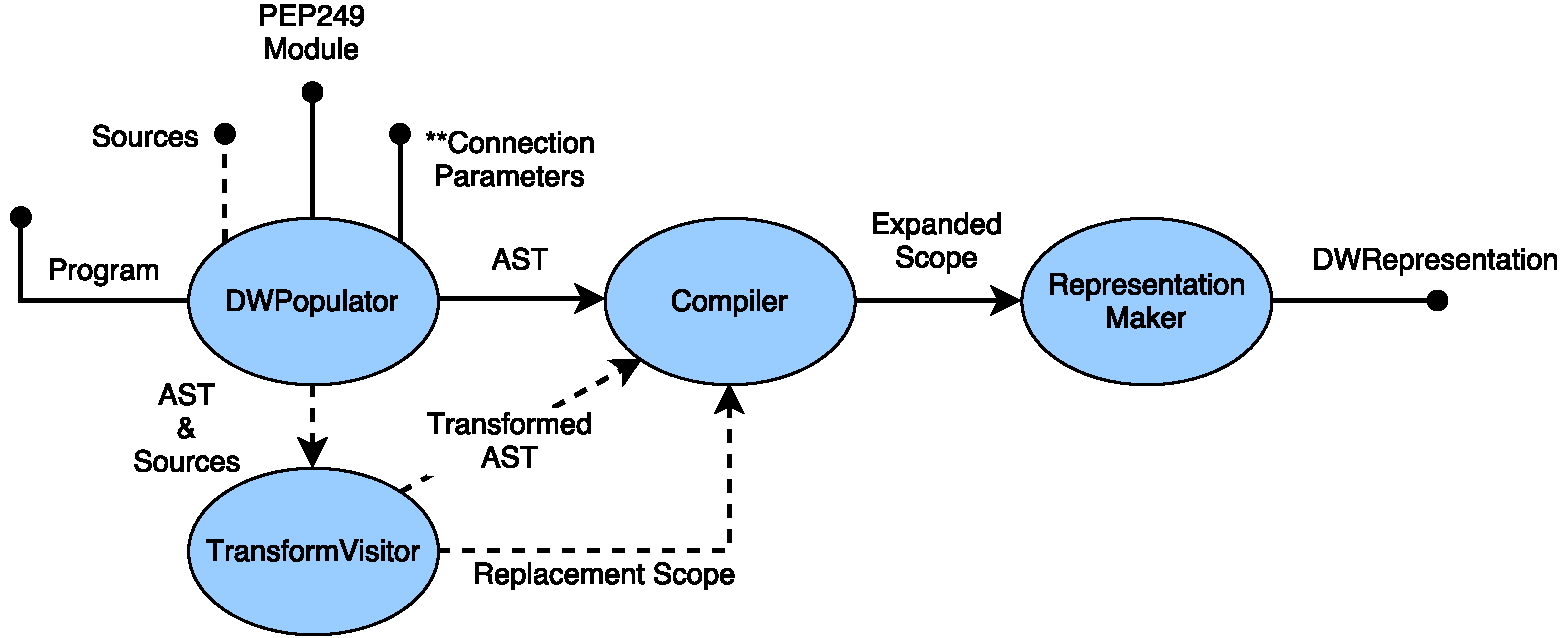
\includegraphics[width=1\textwidth]{figures/reinterpreter.pdf}
  \caption{Data flow diagraml of the Reinterpreter}
  \label{fig:reinterpreter}
\end{figure*}


\section{pygrametl Reinterpreter}
In this section we will describe the purpose and implementation of the reinterpreter component. Its purpose is to make it easier for users to replace the sources and DW in their pygrametl programs. Users may give test sources and DW as input to the reinterpreter, rather than hardcoding them into the program itself. The reinterpreter also outputs a DWRepresentation object, which describes the structure and contents of the DW in question. This object is heavily used by the predicates. On \cref{fig:reinterpreter} is a dataflow diagram that illustrates the flow of data through the reinterpreter. Please note that this depiction is abstracted from the actual implementation as to ease explanation. In the following subsections, we will describe each of the three sub-components shown on the figure.

\subsection{TransformVisitor}
The TransformVisitor takes as input the AST for the pygrametl program being tested, and a replacement scope. The replacement scope is an ordered dictionary. Here we pair dummy keys with objects that connect to  a source or a DW. Such an object can either be a file handle in the case that we access a CVS file, or a PEP249 connection when accessing a database.  TransformVisitor inherits from ast.NodeVisitor and is used to walk over the AST. Each time the visitor encounters a procedure call, it will check whether it is an instantiation of one of the following atomic pygrametl source classes: SQLSource. CSVSource or TypedCVSSource. We label these classes as atomic, as they connect directly to data. Other classes in pygrametl.sources instead encapsulate these classes. Thus, we need only single out these three classes. Once we encounter an instantiation of such a class, the visitor replaces the call parameter that connects to the actual source. This is replaced with a dummy key from our replacement scope.  When another source instantiation is encountered, we replace its parameter with the next key in the scope. After the entire tree has been walked, the transformed AST is finished. This is then sent to the compiler along with the replacement scope. 

\subsection{Compiler}
This is a call to the python compiler, which executes the transformed AST using the replacement scope as its local scope. In python, a scope is given by a dictionary, where keys are variable names paired with object references. As we replaced the connecting objects in the transformed AST with keys from our own scope, we force the program to use the test objects in the replacement scope. This way, we overwrite the hardcoded sources and DW from the program.  Once the AST has been executed, the test DW will be populated, and the replacement scope expanded with the variables found in the script. The expanded scope is sent to the RepresentationMaker. 


\subsection{RepresentationMaker} 
Using the expanded scope, the RepresentationMaker gains access to the Dimension and FactTable objects found within the pygrametl program. These contain a lot of useful information about each table within the DW, such as table names and keys. As database access with pygrametl is done through a PEP249 connection, meta data like this is not easily accessed. Therefore, we use these classes to get a hold of the available meta data . For each atomic Dimension and FactTable object found, we instantiate a DimensionRepresentation or FactTableRepresentation. Again, by atomic we mean that these objects connect directly to a table found in the DW. Each representation object has the purpose of storing meta data and providing access to a specific table. 

Once all tables have been found, we use them to instantiate a DWRepresentation object. This represents the entire DW, and through it all tables can be accessed. During instantiation it also computes and stores the structure of the DW based on primary/foreign key pairs between fact tables and dimensions.  pygrametl requires that a natural join can be made between tables that reference each other. Therefore we base the structure upon matching attribute names between fact tables and dimensions. Once the DWRepresentation object has been instantiated, it is returned from the reinterpreter. Later on it is heavily used by the predicates.